%Style
\documentclass[sn-vancouver,Numbered]{sn-jnl}% Vancouver Reference Style
%\documentclass[sn-apa]{sn-jnl}% APA Reference Style 

%%%% Standard Packages
%%<additional latex packages if required can be included here>

\usepackage{graphicx}%
\usepackage{multirow}%
\usepackage{amsmath}

\usepackage{amsmath,amssymb,amsfonts}%
%\usepackage{amsthm}%
%\usepackage{mathrsfs}%
\usepackage[title]{appendix}%
\usepackage{xcolor}%
\usepackage{textcomp}%
\usepackage{manyfoot}%
\usepackage{booktabs}%
\usepackage{algorithm}%
\usepackage{algorithmicx}%
\usepackage{algpseudocode}%
\usepackage{listings}%
\usepackage{multirow}%
\usepackage{graphicx}

\raggedbottom
\DeclareRobustCommand{\rchi}{{\mathpalette\irchi\relax}}
\newcommand{\irchi}[2]{\raisebox{\depth}{$#1\chi$}}

\usepackage[font=small,skip=7pt]{caption}
\usepackage{orcidlink}
\usepackage{comment}
\usepackage{soul}

\raggedbottom

\begin{document}

\title[Article Title]{SpiNet-QSM: Model-based Deep Learning with Schatten p‐norm Regularization for Improved Quantitative Susceptibility Mapping}

\author[1]{\fnm{Vaddadi} \sur{Venkatesh}}\email{venkateshvad@iisc.ac.in}

\author[2]{\fnm{Raji } \sur{Susan Mathew}}\email{rajisusanmathew@iisertvm.ac.in}

\author*[1]{\fnm{Phaneendra } \sur{K. Yalavarthy}}\email{yalavarthy@iisc.ac.in}

\affil[1]{\orgdiv{Department of Computational and Data Sciences}, \orgname{Indian Institute of Science}, \orgaddress{\city{Bangalore}, \postcode{560012}, \state{Karnataka}, \country{India}}}
\affil[2]{\orgdiv{School of Data Science}, \orgname{Indian Institute of Science Education and Research}, \orgaddress{\city{Thiruvananthapuram}, \postcode{695551}, \state{Kerala}, \country{India}}}

\abstract{Quantitative susceptibility mapping (QSM) provides an estimation of the magnetic susceptibility of tissues from magnetic resonance (MR) phase measurements. Estimation of the tissue magnetic susceptibility (source) from the measured magnetic field distribution/local tissue field (effect) inherent in the MR phase images was achieved by numerically solving the inverse source-effect problem. This work aims to develop an effective model-based deep learning framework to solve the inverse problem of QSM. This work proposes a Schatten $\textit{p}$-norm-driven model-based deep learning framework for QSM with a learnable norm parameter $\textit{p}$ to adapt to the data. In contrast to other model-based architectures that enforce either \textit{l}$_{\textnormal{2}}$-norm or \textit{l}$_{\textnormal{1}}$-norm for the denoiser, the proposed approach can enforce any $\textit{p}$-norm ($\textnormal{0}<\textit{p}\leq \textnormal{2}$) on a trainable regularizer. The proposed method was compared with deep learning-based approaches, such as QSMnet, and model-based deep learning approaches, such as learned proximal convolutional neural network (LPCNN). Reconstructions performed with 77 imaging volumes with different acquisition protocols and clinical conditions, such as hemorrhage and multiple sclerosis, showed that the proposed approach outperformed existing state-of-the-art methods by a significant margin in terms of quantitative merits. The proposed SpiNet-QSM showed a consistent improvement of at least 5\% in terms of the high frequency error norm (HFEN) and the normalized mean squared error (NMSE) over other QSM reconstruction methods in limited training data.}

\keywords{dipole inversion, model-based deep learning, Schatten p-norm, susceptibility reconstruction}

\maketitle
\section{Introduction}\label{sec1}

 Quantitative susceptibility mapping (QSM) is a magnetic resonance imaging (MRI) technique aimed at mapping the magnetic susceptibility of tissue from the gradient echo imaging phase \cite{deistung2017overview,schweser2016foundations,liu2015quantitative,reichenbach2015quantitative}, QSM has important clinical relevance because bulk tissue magnetic susceptibility provides essential information about tissue composition and microstructure, such as myelin content in white matter and iron deposition in gray matter. Pathological changes in these tissue susceptibility sources are closely related to a series of neurodegenerative diseases such as multiple sclerosis and Alzheimer’s disease. Multiple processing steps are involved in obtaining the susceptibility map from the acquired MR data. These  include phase unwrapping, background field removal, and dipole inversion (dipole deconvolution). 

In the first step, the ambiguity caused by the 2$\pi$ periodicity is removed using phase unwrapping. Furthermore, the phase contributions arising from the unwrapped phase due to the air–tissue and air–bone interfaces will be reduced/eliminated in the background field removal because the magnitude of the former component is much larger than that of the tissue component. Some popular background removal techniques are sophisticated harmonic artifact reduction for phase data (SHARP)\cite{schweser2010sophisticated}, regularization enabled SHARP (RESHARP) \cite{sun2014background}, projection onto dipole fields (PDF)\cite{liu2011novel}, spherical mean value (SMV) filtering \cite{wen2014iterative}, Laplacian boundary value background field removal (LBV)\cite{zhou2014background}. The background field removed unwrapped phase is typically referred to as the local field. The following step involves the spatial deconvolution of the dipole kernel with the local field. This is achieved in the Fourier domain by performing an element-wise division between the phase image and the dipole kernel. Owing to the singularity in the dipole kernel, performing a division in the Fourier domain results in an ill-conditioned problem. Thus,  the incorporation of either handcrafted or learned priors is required to efficiently recover the underlying susceptibility map.  

 The advent of deep learning-based methods has shown promising results in deconvolving the susceptibility distribution from the phase information of the MR signal. QSMnet\cite{yoon2018quantitative}, DeepQSM\cite{deepqsm}, and xQSM \cite{Gao2021} are examples of the deep learning approaches developed for computing susceptibility maps. In these methods, a deep neural network was utilized to learn the mapping from the single-orientation phase measurement to the corresponding multi-orientation Calculation of Susceptibility through Multiple Orientation Sampling (COSMOS) \cite{liu2009calculation} susceptibility map, and then utilize the learned network to estimate high-quality susceptibility maps similar to COSMOS from the single-orientation phase measurements. QSMnet uses a three-dimensional convolutional neural network (CNN) U-net \cite{unet} architecture to estimate the susceptibility map. DeepQSM learns the physical forward problem by using synthetic data. To further improve the performance of the QSM reconstruction, octave convolutions were introduced in xQSM \cite{Gao2021}. It also requires end-to-end training from the local field to the COSMOS. 

 Although the aforementioned methods have the potential benefits of deep learning, they do not utilize the underlying physics of the QSM problem and hence are more biased towards the data used for training. Consequently, if the distribution of the input phase data differs from that of the trained data, these methods fail to adapt to the given input, resulting in suboptimal reconstruction. This is aggravated if the model is trained with less data. To alleviate this, model-based deep learning approaches were utilized that combine the power of deep learning and the underlying physics of the problem \cite{MoDL}. Learned proximal convolutional neural network for quantitative susceptibility mapping (LPCNN)\cite{lai2020learned} and model-based deep learning for QSM (MoDL-QSM) are examples of such approaches which were developed for QSM reconstruction. LPCNN approach is an unrolled iterative model that combines the proximal gradient algorithm and a CNN (3D-WideResNet). LPCNN decouples the forward model and data-driven parameters in the reconstruction algorithm. It utilizes a proximal operator parameterized by CNN, which functions as a data-driven regularizer. This regularizer restricts the set of possible solutions by enforcing the prior knowledge. Another model-based approach for QSM reconstruction is MoDL-QSM \cite{modl_qsm}, in which the principal component of susceptibility is utilized as the ground truth or label. 

 In this work, the proposed SpiNet-QSM model introduces a novel deep learning architecture that replaces the traditional $l_2$-norm or $l_1$-norm regularizers with a learnable $p$-norm ($0<p\leq2$) based regularizer, which is automatically learned from the data. The main contributions of this work are : (i) It provides an improved susceptibility map even on limited training data. (ii) It provides better generalizability across different QSM datasets and performs consistently well in region of interest (ROI) analysis. Reconstructions performed across 77 imaging volumes with different acquisition protocols, and clinical conditions such as hemorrhage and multiple sclerosis showed that the proposed approach outperforms existing state-of-the-art reconstruction methods by a significant margin in all figures of merit.
 
%---------
\section{Methods}\label{sec2}

\subsection{Datasets}\label{sec2sub1}
In this work, six datasets were used. The first dataset was from Seoul National University (SNU), South Korea, (SNU data) which consisted of $60$ volumes collected from 12 healthy subjects, was utilized. The data were acquired at 3T (nine datasets using Tim Trio and three datasets using MAGNETOM Skyra, Siemens Healthineers, Forchheim, Germany) at five different head orientations \cite{qsm_net}. The data had dimensions of $176 \times 176 \times 160$. The second dataset was shared by Lai et al. \cite{lai2020learned} (LPCNN data) which consisted of four healthy subjects, acquired at 7T (Philips Achieva) with four head orientations each, with a total of 16 volumes. The data had dimensions of $224 \times 224 \times 126$. The third dataset was shared by reconstruction challenge-1 (RC-1) \cite{langkammer2018quantitative} which consisted of $1$ volume collected from acquired at 3T (Tim Trio, Siemens Healthcare GmbH, Erlangen, Germany) with twelve head orientations. The data had dimensions of $160 \times 160 \times 160$. The fourth dataset was shared by reconstruction challenge-2 (RC-2) \cite{marques2021qsm} simulation2 which consisted of $2$ volumes (sim2snr1,sim2snr2). The data had dimensions of $ 164\times205  \times205 $. For clinical study on hemorrhage and multiple sclerosis, datasets acquired on 3T GE HDxt MR scanner was utilized as shared by \cite{modl_qsm}. These datasets had dimensions $256 \times 256 \times 66$ and $256 \times 256 \times 124$, respectively. All datasets were pre-processed and shared by the respective authors. 

The SNU data was used for training the model. For training, the local field was provided as an input to all methods, and the rotated COSMOS maps that matched the orientation of the input local field were used as the ground truth. To increase the size of the training data, the COSMOS maps were rotated at angles ($-30^{\circ}$ and $30^{\circ}$ relative to $B_{0}$ ), and local field maps were generated by dipole convolution. Using this data augmentation process, the total training data was tripled. Because the QSM problem has been defined in 3D, multiple 3D patches were generated for the training process with a size $64 \times 64 \times 64$ voxels and 66 \% overlap with adjacent patches. The COSMOS map was used as a label/ground truth for all methods considered in this work.

\subsection{QSM reconstruction model }

The relation between the susceptibility map $\rchi \in X$ and the local field $y \in Y$, with $X$ and $Y$ representing the susceptibility and phase spaces, can be expressed as


\begin{equation}
\label{qsm_problem}
    \phi \rchi=y
\end{equation}


\noindent where $\phi =F^HDF$ is the forward operator. Here, $F$ is the discrete Fourier transform and $D$ is the dipole kernel, which is a diagonal matrix. However, there are zeros in $D$, $\rchi$ cannot be computed using a direct inverse and requires the introduction of some prior information about the underlying susceptibility map. In this work, a Schatten $p$-norm prior with $0<p\leq2$ was utilized in a model-based deep learning framework for QSM reconstruction. 

\subsection{SpiNet}
\begin{figure*}[htbp]
    \centering
    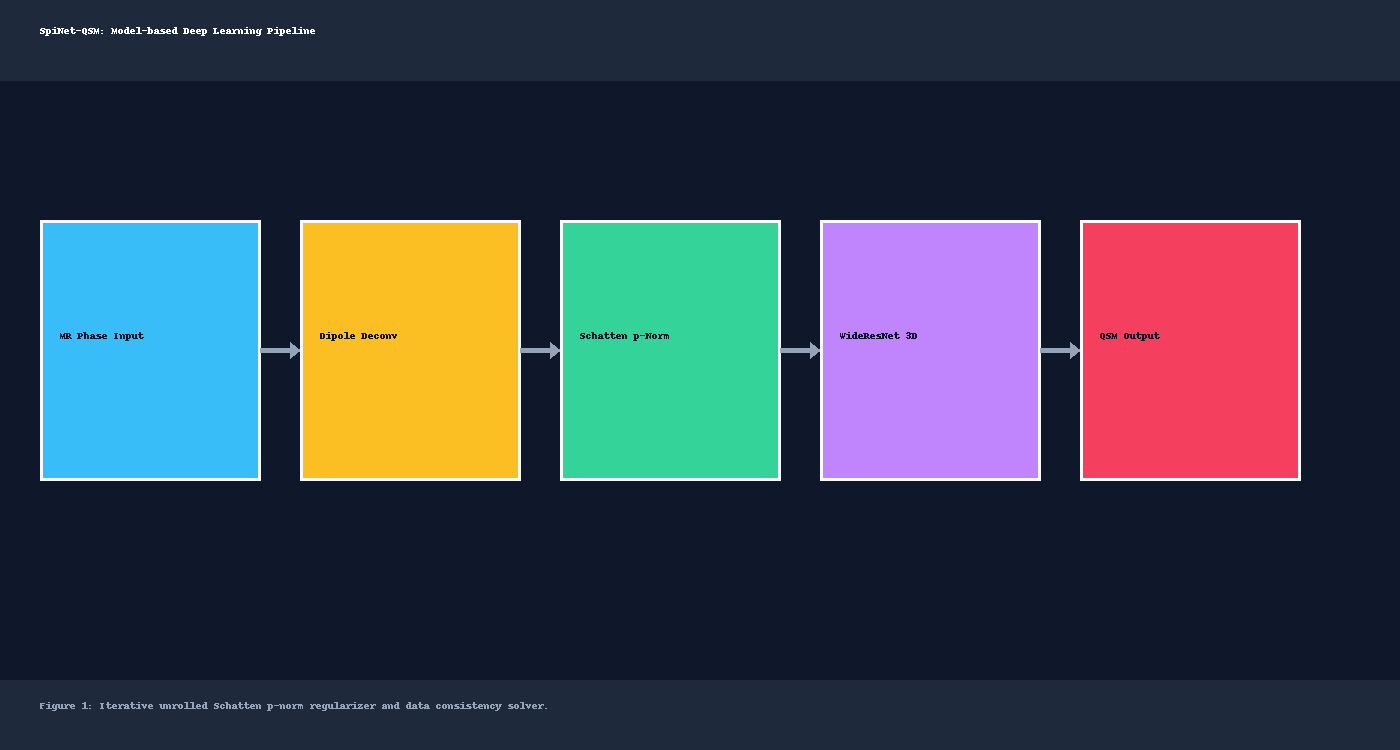
\includegraphics[scale=0.095]{images/fig_1.png}
    \caption{
    (a) Network architecture of the proposed SpiNet-QSM. Each iteration of the network consists of two blocks, namely CNN-denoiser (${D_w}$) block and data consistency block (DC) (b) Proposed SpiNet-QSM has been shown as an unrolled iterative architecture. The bottom row shows the reconstructed susceptibilty maps with iteration for an example case. The respective high-frequency error norm (HFEN) computed with respect to COSMOS shown below the respective susceptibility map shows considerable improvement with iteration.
}
    \label{fig:spinet_qsm_architecture}
\end{figure*}
SpiNet is a model-based deep learning technique for solving the inverse problem with an iterative unrolled structure \cite{Rastogi2021}. It has two parts: the first is a $p$-norm-enforced regularizer with a CNN-based learnable denoiser, and the second is an iterative data consistency solver. SpiNet solves the inverse problem ($Ax=b$) by formulating the following optimization problem:


%\begin{equation}
%\label{spinet_formulating_eqn4}
%\centering    
%x^{*}= \arg \min_{x} \{J(x)=\|Ax-b\|_{2}^{2}+ \lambda \|x-z\|_{p}^{p}\}.
%\end{equation}

\textcolor{black}{
\begin{equation}
\label{spinet_optimization_equation}
x^* = \arg \min_{x} \{ J(x) = \underbrace{\|Ax - b\|^2_2}_{\text{Data Consistency Term}} + \underbrace{\lambda \|x - z\|^p_p}_{\text{Prior Information Enforcing Term}} \}
\end{equation}}
\textcolor{black}{where}


\textcolor{black}{
\begin{equation}
\label{spinet_optimization_equation_2}
z=D_{w}(x)
\end{equation}}

\noindent
\textcolor{black}{Here, the eq.(\ref{spinet_optimization_equation}), $\|Ax - b\|^2_2$ represents the data consistency term, and $\|x - z\|^p_p$ represents the regularization term, with $\lambda$ denoting the regularization parameter that balances the trade-off between the data consistency term and the regularization term. Here $z$ in eq.(\ref{spinet_optimization_equation_2}) is a denoised version of x, which is an output of the CNN-based denoiser denoted by $D_w$, and eq. ~ (\ref{spinet_optimization_equation}). The solution $x^{*}$ is constrained to follow data consistency and is in the vicinity of $z$. The solution $x^{*}$ simultaneously minimizes the data consistency term $\|Ax - b\|^2_2$ and considers the prior information through the regularization term, which comprises the CNN-based denoiser.}


\noindent
The eq. (\ref{spinet_optimization_equation}) is solved by utilizing the majorization-minimization (MM) approach. This consists of two steps: computing the convex upper bound function $\mathcal{F}(x)$ (majorization) and solving the upper bound function (minimization) in an iterative manner. The steps involved in solving SpiNet are as follows:

\vspace{1mm}
\begin{equation}
\label{spinet_formulating_z_defined}
\centering    
z_{k}=D_w(x_{k-1})
\end{equation}
\vspace{-1mm}
\begin{equation}
\label{spinet_formulating_F_defined_1}
    (W_{k})_{ii}=|(\bar{x})_{i}-(z_{k})_{i}|^{p/2-1}
\end{equation}
\vspace{-1mm}
\begin{equation}
\label{spinet_formulating_F_defined_2}
\centering    
   \mathcal{F}(x) = \|Ax-b\|_{2}^{2}+ \lambda^{'} \|W_{k}(x-z_{k})\|_{2}^{2} \geq J(x)
\end{equation}
\vspace{-1mm}
\begin{equation}
\label{spinet_formulating_minimization_1}
\centering
   x_{k}=\arg \min_{x} \|Ax-b\|_{2}^{2}+ \lambda^{'} \|W_{k} (x-z_{k})\|_{2}^{2}
\end{equation}
\vspace{-1mm}
\begin{equation}
\label{spinet_formulating_minimization_2}
\centering
   x_{k}=(A^{H}A+\lambda^{'}W_{k}^{H}W_{k})^{-1}(A^Hb+\lambda^{'}W_{k}^{H}W_{k}z_{k})
\end{equation}
\vspace{1mm}
\noindent where $\bar{x}$ is the known point nearer to the $x^{*}$ at the $k^{th}$ iteration (in the implementation the $x_{k-1}$ is used as $\bar{x}$), $W_k$ is a diagonal matrix and $\lambda^{'}=\lambda p/2$.
Here, eq. (\ref{spinet_formulating_z_defined}), eq. (\ref{spinet_formulating_F_defined_1}) and eq. (\ref{spinet_formulating_F_defined_2}) represents the majorization step and eq. (\ref{spinet_formulating_minimization_1}) and eq. (\ref{spinet_formulating_minimization_2}) are represent the minimization step. The minimization step in eq. (\ref{spinet_formulating_minimization_2}), is solved using the conjugate gradient (CG) method to estimate $x_{k}$ given $W_{k}$ and $z_{k}$. The output $x_{k}$ from the minimization step was used as $\bar{x}$ for the majorization step in the $(k+1)$th iteration. The denoisers share weights across all iterations with end-to-end learning, which effectively reduces the number of learnable parameters \cite{MoDL}.


\textcolor{black}{All the steps from eq. (\ref{spinet_formulating_z_defined}) to eq. (\ref{spinet_formulating_minimization_2}) were considered as a single unrolling step. However, this method makes an end-to-end network by unfolding the data consistency block and denoiser block interleaved manner for $K$ times. Here, $K$ is known as the unrolling parameter. These interleaved CNN blocks, learn the prior information from the dataset set, along with data consistency blocks that constrain the reconstruction to follow the physics of the problem. }
\subsection{Proposed SpiNet-QSM}

To adopt SpiNet to QSM reconstruction problem, eq. (\ref{qsm_problem}) was redefined with a Schatten p-norm enforced regularizer,  


\begin{equation}
    \label{qsm_spinet_formulation_1}
\rchi^{*}= \arg \min_{\rchi}  \{\bar{J}(\rchi)=\left \| \phi \rchi - y\right \|_{2}^{2}+\lambda \left \| \rchi -z \right \|_{p}^{p}\}
\end{equation}

\noindent Now, $\bar{J}(\rchi)$ can be iteratively solved using the majorization-minimization approach as described earlier. The upper bound function of $\bar{J}(\rchi)$ denoted as $\bar{\mathcal{F}}(\rchi)$ is first defined (majorization step) by taking an analogy from  eq. (\ref{spinet_formulating_z_defined}), eq. (\ref{spinet_formulating_F_defined_1}) and eq. (\ref{spinet_formulating_F_defined_2}) as

\begin{equation}
\label{qsm_spinet_formulation_majorization_1}
z_k=D_w(\rchi_{k-1})
\end{equation}
\vspace{-1mm}
\begin{equation}
\label{qsm_spinet_formulation_majorization_3}
    (W_{k,j})_{ii}=|(\bar{\rchi}_{k,j-1})_{i}-(z_{k})_{i}|^{\frac{p}{2}-1} \\ \hspace{2mm} 
\end{equation}
here, $\bar{\rchi}_{k,0}=\rchi_{k-1}.$
\begin{equation}
\label{qsm_spinet_formulation_majorization_2}
 \bar{\mathcal{F}}(\rchi)=\left \| \phi \rchi - y\right \|_{2}^{2}+\lambda \left \| W_{k,j}(\rchi -z_{k}) \right \|_{2}^{2} 
\end{equation}
\noindent where $z_{k}$ is the denoised susceptibility map which is obtained from eq. (\ref{qsm_spinet_formulation_majorization_1}) by taking input as $\rchi_{k-1}$ and, $\bar\rchi_{k,j}$ is a calculated susceptibility map in $j^{th}$ step of the MM in $k^{th}$ iteration. The minimization step (solving upper bound function $\bar{\mathcal{F}}(\rchi)$ ) was defined by taking the analogy from the eq. (\ref{spinet_formulating_minimization_1}) and eq. (\ref{spinet_formulating_minimization_2}) and it showed as

\begin{equation}
\label{spinet_qsm_formulating_minimization_1}
\bar\rchi_{k,j}=\arg \min_{\rchi}\{\bar{\mathcal{F}}(\rchi)\}
\end{equation}
% \{\bar{F}(\rchi)=\left \| \phi \rchi - y\right \|_{2}^{2}+\lambda \left \| W_{k,j}(\rchi -z_{k}) \right \|_{2}^{2}\}
\vspace{-1mm}
\begin{equation} 
\label{spinet_qsm_formulating_minimization_2}
    \bar\rchi_{k,j}=(\phi ^{H} \phi +\lambda W_{k,j}^{H}W_{k,j})^{-1}(\phi ^{H} y +\lambda W_{k,j}^{H}W_{k,j} z_{k})
\end{equation}
\vspace{1mm}
\noindent  Here, the eq. (\ref{spinet_qsm_formulating_minimization_1}) can be solved using normal equations eq. (\ref{spinet_qsm_formulating_minimization_2}). Now, this can be solved using a CG solver of $\bar A x=\bar b$.

\begin{equation}
\scriptsize
\bar{A}=(\phi ^{H} \phi +\lambda W_{k,j}^{H}W_{k,j})=(F^HD^2F+\lambda W_{k,j}^HW_{k,j})
\end{equation}
\vspace{-1mm}
\begin{equation}
\scriptsize
\bar{b}=(\phi ^{H} y +\lambda W_{k,j}^{H}W_{k,j} z_{k})=(F^HDFy+\lambda W_{k,j}^HW_{k,j}z_{k})        
\end{equation}
\vspace{1mm}
\noindent At each iteration, this results in performing majorization and minimization $N$ times and the susceptibility map output from $k^{th}$ iteration is $\rchi_{k}=\bar\rchi_{k,N}$. A detailed $k^{th}$ step-wise explanation of QSM solving using SpiNet is provided in Algorithm (\ref{alg:spinet_qsm_algorithm}).

\begin{algorithm}[!t] 
\scriptsize
\caption{Algorithm for proposed Spinet-QSM}
\label{alg:spinet_qsm_algorithm}
\begin{algorithmic}[1]
\Require Local field ($y$), No of Unrollings ($K$), No of MM-steps ($N$)

\State $\rchi_{0}={\phi}^{H}y$
\State $\textbf{for} \hspace{1mm} k=1 \hspace{1mm} to \hspace{1mm} K \hspace{1mm} \textbf{do}$
\State $\hspace{3mm} z_k=Dw(\rchi_{k-1})$
\State $\hspace{3mm} \bar{\rchi}_{k,0}=\rchi_{k-1}$
\State $\hspace{3mm} \textbf{for} \hspace{1mm} j=1\hspace{1mm}to\hspace{1mm}N\hspace{1mm} \textbf{do}$
\State $\hspace{6mm}(W_{k,j})_{ii}=|(\bar\rchi_{k,j})_{i}-({z}_{k})_{i}|^{\frac{p}{2}-1} $
\State $\hspace{6mm}\bar{\rchi}_{k,j}= (\phi ^H\phi +\lambda W_{k,j}^{H}W_{k,j})^{-1}(\phi ^H 
y+\lambda W_{k,j}^{H}W_{k,j} z_{k})$
\State $\hspace{3mm}\textbf{end for}$
\State $\hspace{3mm}{\rchi}_{k}=\bar{\rchi}_{k,N}$
\State $\textbf{end for}$

\end{algorithmic}
\end{algorithm}



\begin{table*}[htbp]
\centering
\caption{\textcolor{black}{Summary of the training parameters for different models utilized in this study.}}
{\small
\begin{tabular}{|lllccc|}
\hline
\textbf{Experiment} 
&  \textbf{Learning Rate}
& \textbf{Loss function }
& \textbf{Batch size} 
& \textbf{\shortstack{No. of Epochs \\Trained}} 
& \textbf{\shortstack{Time taken for \\single epoch (Minutes)}} \\
\hline

SpiNet-QSM
&  $1\times 10^{-4}$ & $w_{1}(loss_{L1})+w_{2}(loss_{Gradient})$ 
& 2 
& 45 
& 90 \\

LP-CNN 
&  $1\times 10^{-4}$ 
& $w_{1}(loss_{L1})+w_{2}(loss_{Gradient})$ 
& 2
& 80 
& 120\\

QSMNet 
&  $5\times 10^{-4}$ & $w_{1}(loss_{L1})+w_{2}(loss_{Gradient})$ 
& 8 
& 25 
& 30\\

DeepQSM 
&  $5\times 10^{-4}$ 
& $loss_{L2}$ 
&  8 
& 25 
& 30\\

xQSM 
&  $5\times 10^{-4}$ 
& $loss_{L2}$ 
& 8 
& 25 
& 50\\

\end{tabular} }
\label{tab:updated_experimental_details}
\end{table*}

%% figure 2 
\begin{figure}[htbp]
\centering
   \scalebox{1}{
    %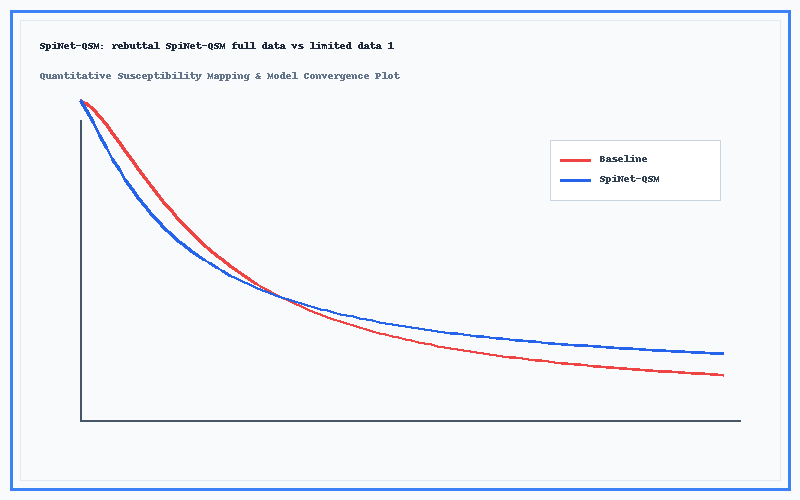
\includegraphics[width=\linewidth]{rebuttal_images/rebuttal_SpiNet-QSM_full_data_vs_limited_data_1.png}
    }
    
    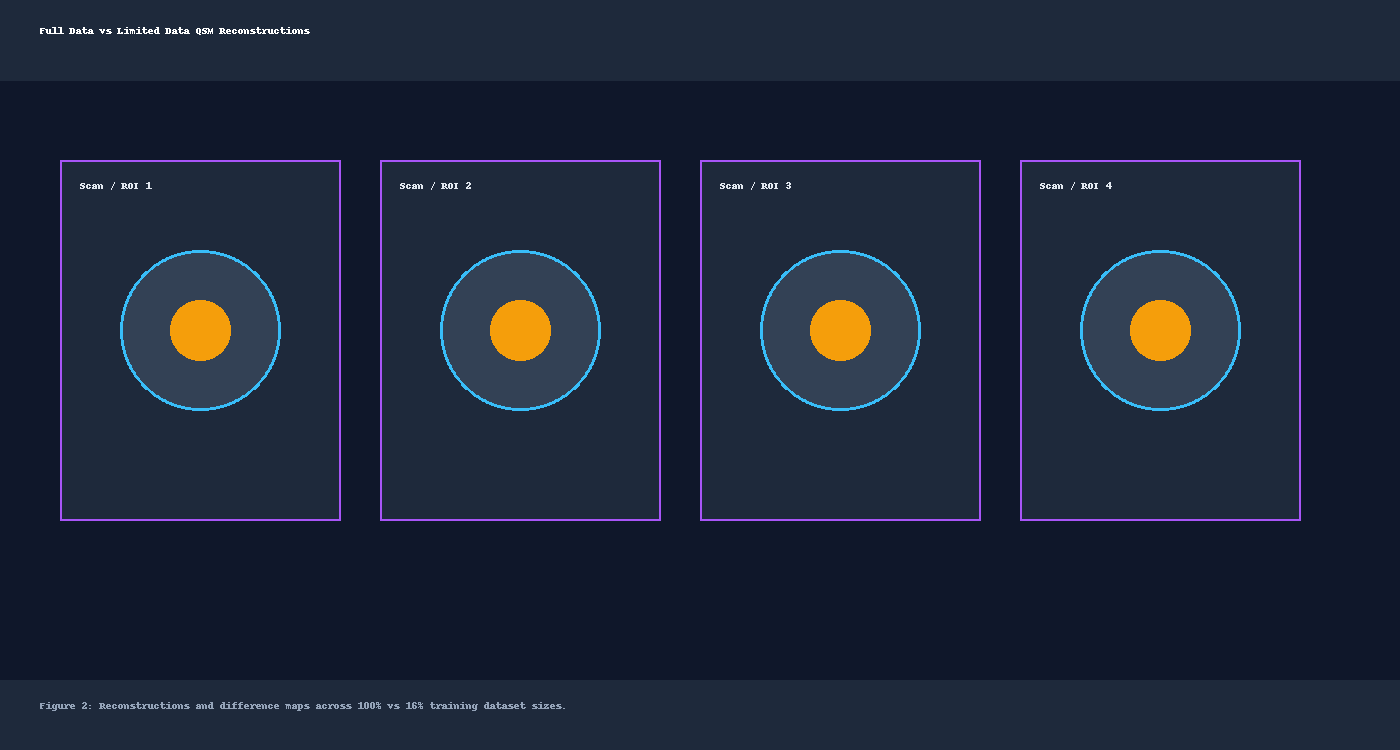
\includegraphics[scale=0.33]{rebuttal_images/rebuttal_SpiNet-QSM_full_data_vs_limited_data_2.png}
    \caption{\textcolor{black}{(a) An example susceptibility image reconstructed using the complete data training was shown in the first row, and the difference images with respect to COSMOS in the second row.  (b) The same data reconstructed on limited data training (16\% of the data utilized in (a)) are shown in the first row, and the difference images with respect to COSMOS are shown in the second row. The corresponding high-frequency error norm (HFEN) and normalized mean squared error (NMSE) with respect to COSMOS are shown below the respective susceptibility map and difference image, respectively. As NDI is an iterative method, the reconstruction results (NMSE=57.734 and HFEN=54.175) were not included in the figure.}}
    \label{fig:qsm_maps_on_complete_vs_limited}
\end{figure}
\subsection{Proposed SpiNet-QSM architecture}
The proposed SpiNet-QSM architecture is shown in Fig. \ref{fig:spinet_qsm_architecture}. It has two blocks: a regularizer that consists of a CNN-based denoiser for eq. (\ref{qsm_spinet_formulation_majorization_1}), and another one is a data consistency block for eq. (\ref{spinet_formulating_minimization_1}). In the data consistency block, MM implementation is performed utilizing eq. (\ref{qsm_spinet_formulation_majorization_1}) to eq. (\ref{qsm_spinet_formulation_majorization_2}). In the Minimization step, CG method was utilized to solve eq. (\ref{qsm_spinet_formulation_majorization_2}) with $M_1=25$ iterations to estimate $\rchi$ given $W$ and $z_{k}$, and use this $\rchi$ as $\bar{\rchi}$ for the next Majorization step. The MM algorithm is repeated for $N=2$ iterations. The denoiser block ($D_{w}$) uses a 3D-WideResNet CNN architecture inspired by Refs. [\cite{lai2020learned,he2016deep}]. This is an implicit data-driven regularizer that uses the power of residual learning. It has $21$ convolutional layers and eight repetitive residual blocks. For the first 17 convolutional layers, the kernel size was $3 \times 3 \times 3$ with a stride of one, and for the last three convolutional layers, the kernel size was $1 \times 1 \times 1$ and stride 1. Batch normalization layer (BN) and rectified linear unit (ReLU) activation functions were utilized inside the residual blocks. The last layer of the network is a convolutional layer with a kernel size of one. In the proposed SpiNet-QSM network, the trainable parameters are $\theta=\{\lambda _{i},(D_{w})_{i},p_{i}\}_{i=1}^{K}$, where $K$ is the number of iterations in the unrolled network. However, the training parameters were shared among different iterations. Therefore, the training parameters are $\theta=\{\lambda ,D_w,p\}$.


\subsection{Implementation}

The proposed SpiNet-QSM was implemented using Python 3.9.12 and PyTorch 1.11.0. It was trained on an NVIDIA Quadro RTX 8000 graphics processing unit (GPU). 
\noindent \textcolor{black} {For all deep learning models in this work, Adam optimizer is utilized. The other training parameters, including the learning rate, loss function, batch size, number of epochs, and time for each epoch, are summarized in Table \ref{tab:updated_experimental_details}. It is to be noted that the training parameters for each model was chosen empirically so as to give the best performance on the validation data. In Table \ref{tab:updated_experimental_details} the $loss_{L1}$ term is defined as the $l_1$-norm of the voxel-wise difference, and the $loss_{Gradient}$ term is defined as the $l_1$-norm of gradients difference. $w_1$ and $w_2$ are the weights assigned to $loss_{L1}$ and $loss_{Gradient}$ respectively. The weights were chosen as $w1=1$ and $w2=0.5$, determined empirically. The $loss_{L2}$ term is defined as the $l_2$-norm of the voxel-wise difference, and it is nothing but a mean square error between ground-truth and reconstructed QSM.} \textcolor{black}{Further, in the proposed SpiNet-QSM, the number of MMsteps ($N$) was chosen as 2, and the number of CG iterations ($M_1$) was 25; these parameters were empirically selected. It has also experimented with $N \ge 2$ and $M_{1} \ge 25$; however, it did not show any improvement in performance compared to $N=2$ and $M_{1}=25$. Instead, it increased the GPU computation and GPU RAM consumption during training. }


\vspace{8pt}
\textcolor{black}{\subsubsection{Selection of $D_w$}}

\noindent \textcolor{black}{A 3D-WideResNet18 CNN architecture was used as the trainable regularizer. This architecture was empirically chosen by experimenting with different 3D CNN architectures. To choose $D_w$, a simple residual-learning-based 3D CNN architecture (with five layers) was initially used, motivated by MoDL \cite{MoDL}. As QSM reconstruction is a challenging 3D problem, the regularizer faces underfitting issues when trained on complete data. When 3D-UNet was used as the regularizer, it performed well on the complete training data with K=1. However, it did not show any improvement for $K=2$ and 3. The 3D-Unet architecture performed poorly as a learning regularizer with shared weights over iterations, and thus cannot use the advantage of the unrolled structure. This architecture also faces an underfitting issue when trained with limited data. Finally, the 3D WideResNet18 architecture was utilized as a trainable regularizer. It performed well on complete and limited training data, and showed improved reconstruction for $K>1$.}


\textcolor{black}{\subsubsection{Selection of $K$}}
\noindent \textcolor{black}{In general, training any model-based deep learning technique is more challenging than training pure deep learning techniques, requiring additional training time. The proposed SpiNet-QSM has an unrolled architecture with shared weights and requires additional effort to train the CNN regularizer. To arrive at the optimal value of the number of iterations ($K$), experiments were performed with different unrolling parameters, i.e., $K=1,2,3,$ and $4$. It was observed that the reconstruction performance improved as the number of iterations increased from 1 to 2 and 2 to 3. However, from 3 to 4, this did not lead to significant improvement and made the training process more difficult in terms of delayed convergence and increased training time. As the number of iterations increases, learning a common regularization term across the inputs and outputs in each iteration becomes more difficult, owing to the sharing of weights across iterations. This implies that for $K>3$, the CNN complexity is insufficient to learn the QSM problem with shared weights. However, if one increases the complexity of CNN and the number of iterations ($K>3$) then the training process becomes more difficult. The proposed SpiNet-QSM showed the best performance at $K=3$, and therefore, $K=3$ was fixed as the number of unrolling iterations in all the experiments.}\\

\subsection{Experiments}
\subsubsection{Effect of Dataset Size }
\textit{Training on complete data:} Out of the 12 healthy volunteer scans from SNU data, each with five head orientations, 25 scans from five subjects (along with augmented data consisting of 75 scans) were utilized for training, five scans from one subject were used for validation, and 30 scans from six subjects were utilized for testing. A 4-fold cross-validation was performed. In order to compare SpiNet-QSM with other popular deep learning models, QSMnet, DeepQSM, xQSM and \textcolor{black}{LPCNN} were also trained to solve QSM. \textcolor{black}{As the outcomes of the second QSM reconstruction challenge \cite{qsm2021qsm} revealed that while deep learning methods often produce visually appealing results, their quantitative performance is generally inferior to that of iterative methods, the deep learning methods were also compared with an iterative method. Among the different state-of- the- art nonlinear iterative reconstruction methods such as nonlinear dipole inversion (NDI) \cite{polak2020nonlinear}, fast nonlinear susceptibility inversion (FANSI)\cite{milovic2018fast} and nonlinear total field inversion \cite{nguyen2020quantitative}, NDI was used for comparison in this study.} For the deep model training, 4-fold cross-validation is used.


\noindent \textit{Training on limited data:} An experiment involving a comparison of the reconstruction performances of different methods under a limited data setting was also performed. Here, the training dataset consisted of a single subject's data (along with augmented data consisting of 15 scans), the validation (same as that of full data training) set consisted of single subject data, and the test set consisted of ten subject's data. Single subject data was utilized in this experiment, which is approximately 16\% of that of `the training on complete data.' The training settings detailed in the preceding section were used for the deep learning models even when dealing with limited data training.


\begin{figure}[htbp]
    \centering
    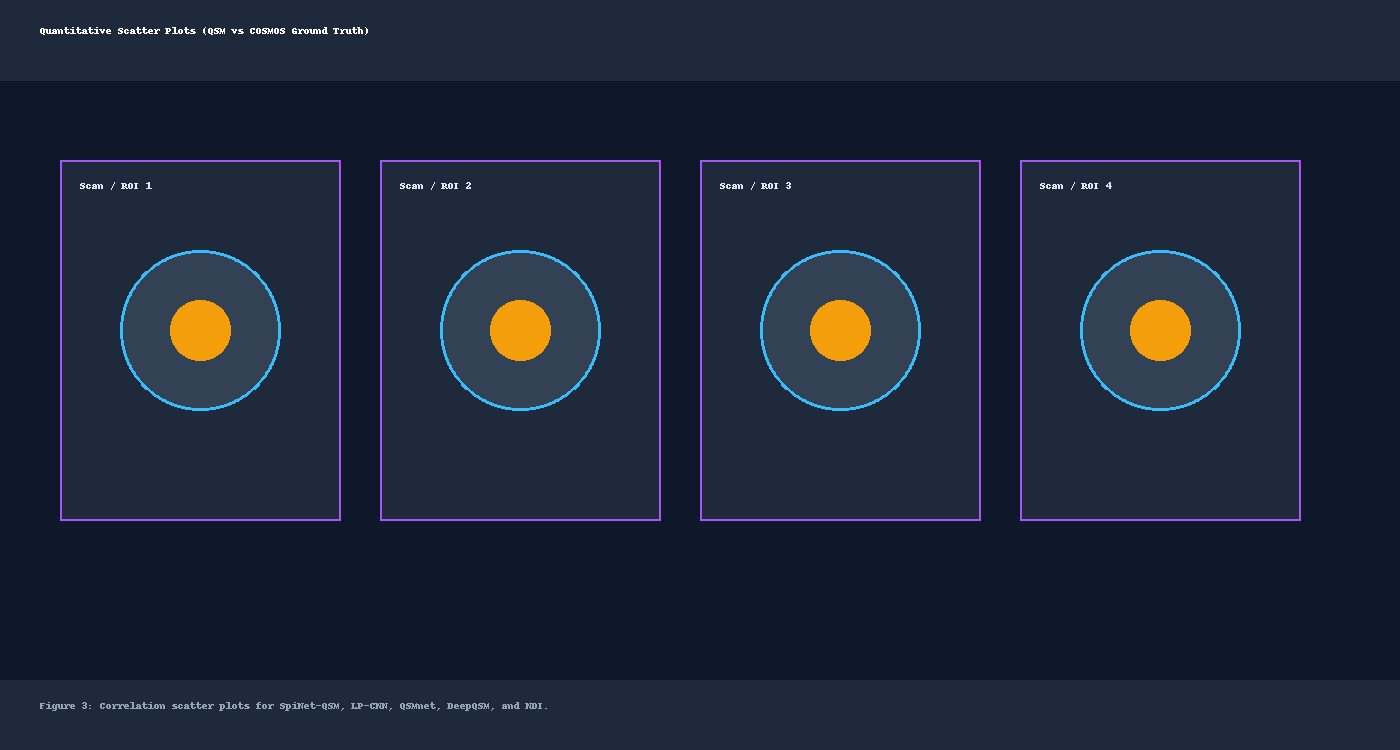
\includegraphics[scale=0.44]{rebuttal_images/scatter_plots_updated.png}
    \caption{
(a) Scatter plots of QSM maps reconstructed using the proposed SpiNet-QSM, LP-CNN, QSMnet, DeepQSM, and xQSM, which were trained on complete training data. (b) Scatter plots of  QSM maps reconstructed using the same five methods and trained on limited training data. QS represents the quantitative susceptibility value in parts per million (ppm). As NDI is an iterative method, the same scatter plot was included in both scenarios and is showcased as a sixth figure}
    \label{fig:scatterplots}
\end{figure}


%% table
\begin{table*}[htbp]
\centering
\caption{\textcolor{black}{Averaged quantitative performance metrics (SSIM, pSNR, NMSE, and HFEN) of different QSM reconstruction methods with respect to COSMOS estimated using 4-fold cross-validation set. The best results are shown in bold.}}
{\small
\begin{tabular}{clllll}
\hline
\multirow{2}{*}{\textbf{Experiment}}
&\multirow{2}{*}{\textbf{Method}} 
& \multicolumn{4}{c}{\textbf{METRICS}} \\ \cmidrule{3-6} 
&                       
& \textbf{SSIM}     
& \textbf{pSNR}         
& \textbf{NMSE}       
&\textbf{HFEN}  \\ \cmidrule{1-6} 

\multirow{6}{*}{\textbf{Complete data training}}        
& \textbf{SpiNet-QSM}   
&\textbf{0.904 $\pm$ 0.031}	 
&\textbf{40.296 $\pm$ 1.622}	
&\textbf{54.782 $\pm$ 8.733}	 
&\textbf{52.054 $\pm$ 9.262} \\ 
                                
& LP-CNN                
&0.889 $\pm$ 0.028	 
&39.570 $\pm$ 1.428	
&58.927 $\pm$ 7.758	 
&56.571 $\pm$ 9.152\\ 

& QSMnet                
&0.902 $\pm$ 0.029	 
&40.244 $\pm$ 1.510	
&54.637 $\pm$ 8.118	 
&52.880 $\pm$ 9.587\\ 
                                
& DeepQSM               
 &0.899 $\pm$ 0.029   
 &40.179 $\pm$ 1.470    
 &55.225 $\pm$ 7.944  
 &54.110 $\pm$ 9.277 \\ 

& xQSM                
&0.901 $\pm$ 0.029   
&40.176 $\pm$ 1.519    
&55.293 $\pm$ 8.293
&53.833 $\pm$ 9.545 \\ 

& \textcolor{black}{NDI}                
&\textcolor{black}{0.868 $\pm$ 0.035}
&\textcolor{black}{38.257 $\pm$ 1.351}  
&\textcolor{black}{70.089 $\pm$ 8.228}
&\textcolor{black}{66.152 $\pm$ 8.631}\\
\hline 
\multirow{6}{*}{\textbf{Limited data training}}        
& \textbf{SpiNet-QSM}   
&\textbf{0.895 $\pm$  0.027}     
&\textbf{39.933 $\pm$ 1.453 }	    
&\textbf{57.001 $\pm$ 7.459}	    
&\textbf{54.605 $\pm$ 8.838} \\ 
& LP-CNN                
&0.881$ \pm$ 0.027	            
&39.271 $\pm$ 1.387 	    
&61.794 $\pm$ 6.801	    
&59.316 $\pm$ 8.323 \\ 
& QSMnet                
&0.861 $\pm$ 0.042	            
&38.698 $\pm$ 1.619	    
&65.475 $\pm$ 9.756	    
&68.881 $\pm$ 12.657 \\ 
& DeepQSM               
&0.861 $\pm$ 0.042     	       
&38.723 $\pm$ 1.578        
&65.402 $\pm$ 9.308        
&66.554 $\pm$ 12.142 \\ 
& xQSM                
&0.853 $\pm$ 0.054     	       
&38.590 $\pm$ 1.692        
&66.893 $\pm$ 10.446        
&67.176 $\pm$ 13.096 \\ 
& \textcolor{black}{NDI}                
&\textcolor{black}{0.868 $\pm$ 0.035}
&\textcolor{black}{38.257 $\pm$ 1.351}  
&\textcolor{black}{70.089 $\pm$ 8.228}
&\textcolor{black}{66.152 $\pm$ 8.631}\\
\hline
\end{tabular} }
\label{tab:results_of_full_data_trained_models}
\end{table*}


\subsubsection{Performance on Other Datasets}
To assess the robustness of the model in terms of reconstruction and demonstrate how well the regularization term generalizes the QSM reconstruction problem, the performances of different methods were compared on datasets with different acquisition parameters. These datasets differed from the training data in terms of acquisition parameters, vendors, and signal-to-noise ratio (SNR). For this, the models trained on SNU data were tested using LPCNN data \cite{lai2020learned}, RC-1 data \cite{langkammer2018quantitative} and RC-2 data \cite{marques2021qsm}. \textcolor{black}{ As this experiment was performed to evaluate the generalizability and performance of the trained models on unseen data, we did not use any type of pre-processing before reconstructing the respective data. It should be noted that the models trained on complete data were used in this experiment.}

\begin{table*}[htbp]

\centering
\caption{\textcolor{black}{Quantitative metrics with respect to COSMOS obtained by testing on other data sets (LP-CNN data, RC-1 data and RC-2 (Sim2Snr1 and Sim2Snr)) data\cite{qsm2021qsm}. The models were trained on SNU data. The best results are shown in bold font. As NDI is an iterative method, results for RC-1 and RC-2 data were presented without standard deviation (No cross-validation). }}
{\small

\begin{tabular}{clllll}
\hline
\multirow{2}{*}{\textbf{Experiment}}
&\multirow{2}{*}{\textbf{Method}} 
&\multicolumn{4}{c}{\textbf{METRICS}} \\ \cmidrule{3-6}
&                       
& \textbf{SSIM}     
& \textbf{pSNR}         
& \textbf{NMSE}       
&\textbf{HFEN}  \\ \hline
\multirow{5}{*}{\textbf{LPCNN data}}        
& \textbf{SpiNet-QSM}   
&\textbf{0.927 $\pm$ 0.013}	    
&\textbf{35.071 $\pm$ 1.480}	    
&\textbf{57.340 $\pm$ 2.912}	  
&\textbf{53.533 $\pm$ 3.472} \\ 

& LP-CNN                
&0.914 $\pm$ 0.011              
&34.651 $\pm$ 1.537	              
&61.353 $\pm$ 2.318                 
&56.931 $\pm$ 2.875\\ 
& QSMnet                
&0.918 $\pm$ 0.014	      
&34.612 $\pm$ 1.498	     
&61.046 $\pm$ 2.879         
&56.422 $\pm$ 3.792\\ 
& DeepQSM               
&0.918 $\pm$ 0.0128	     
&34.693 $\pm$ 1.592
&61.202 $\pm$ 2.662
&56.669 $\pm$ 3.409\\ 

&\textcolor{black}{ xQSM}               
&\textcolor{black}{0.917 $\pm$ 0.011}	     
&\textcolor{black}{34.580 $\pm$ 1.275}
&\textcolor{black}{61.443 $\pm$ 2.554}
&\textcolor{black}{57.301 $\pm$ 3.243}\\ 



\hline

\multirow{6}{*}{\textbf{RC-1 data}}     
&\textbf{SpiNet-QSM}    
&\textbf{0.916 $\pm$ 0.003}	    
&\textbf{40.653 $\pm$ 0.299}	    
&\textbf{47.150 $\pm$ 0.392}      
&\textbf{46.0752 $\pm$ 0.539}\\  

& LP-CNN                
&0.900 $\pm$ 0.002	    
&39.492 $\pm$ 0.124
&52.217 $\pm$ 0.531	  
&49.970 $\pm$ 0.381\\ 

& QSMnet                
&0.909 $\pm$ 0.002      
&39.764 $\pm$ 0.254
&51.545 $\pm$ 1.491
&49.225 $\pm$ 1.177\\  

& DeepQSM               
&0.908 $\pm$ 0.004	            
&39.601 $\pm$ 0.280	                
&52.076 $\pm$ 0.743	              
&50.175 $\pm$ 1.040\\ 

&\textcolor{black}{ xQSM}               
&\textcolor{black}{0.909 $\pm$ 0.003}	     
&\textcolor{black}{39.560 $\pm$ 0.276}
&\textcolor{black}{52.577 $\pm$ 0.713}
&\textcolor{black}{50.133 $\pm$ 1.073}\\ 

&\textcolor{black}{ NDI}                              
&\textcolor{black}{0.853}	     
&\textcolor{black}{37.457}
&\textcolor{black}{61.715}
&\textcolor{black}{60.728}\\


\hline

\multirow{6}{*}{\textbf{RC-2 (Sim2Snr1)}}     
&\textbf{SpiNet-QSM}    
&\textbf{0.991 $\pm$ 0.0002 }	    
&\textbf{51.336 $\pm$ 0.138}	    
&\textbf{54.187 $\pm$ 1.527}      
&50.076 $\pm$ 0.995\\  

& LP-CNN                
&0.991 $\pm$ 0.0005	    
&51.057 $\pm$ 0.226
&56.424 $\pm$ 0.391	  
&51.695 $\pm$ 1.053\\ 

& QSMnet                
&0.987 $\pm$ 0.001      
&49.318 $\pm$ 0.376
&66.525 $\pm$ 1.752
&58.186 $\pm$ 3.206\\  

& DeepQSM               
&0.987 $\pm$ 0.001	            
&49.477 $\pm$ 0.316	                
&67.731 $\pm$ 1.264	              
&60.366 $\pm$ 1.567\\ 

& xQSM               
&0.987 $\pm$ 0.001	     
&49.168 $\pm$ 0.291
&67.459 $\pm$ 1.532
&59.363 $\pm$ 1.208\\ 

& NDI                              
&0.984	     
&51.056
&55.384
&\textbf{48.661}\\ 
\hline

\multirow{6}{*}{\textbf{RC-2 (Sim2Snr2)}}     
&\textbf{SpiNet-QSM}    
&\textbf{0.991 $\pm$ 0.0004}	    
&\textbf{51.300 $\pm$ 0.367}	    
&53.073 $\pm$ 1.688
&49.253 $\pm$ 0.989\\  

& LP-CNN                
&0.991 $\pm$ 0.0004	    
&50.968 $\pm$ 0.209
&55.377 $\pm$ 0.667	  
&50.816 $\pm$ 1.260\\ 

& QSMnet                
&0.987 $\pm$ 0.002  
&49.305 $\pm$ 0.421
&65.882 $\pm$ 2.036
&57.436 $\pm$ 3.274\\  

& DeepQSM               
&0.987 $\pm$ 0.001	            
&49.293 $\pm$ 0.277	                
&67.301 $\pm$ 1.347	              
&59.893 $\pm$ 1.687\\ 

& xQSM               
&0.987 $\pm$ 0.001	     
&49.130 $\pm$ 0.197
&67.052 $\pm$ 1.801
&58.892 $\pm$ 1.311\\ 

& NDI                              
&0.987	     
&51.385
&\textbf{52.560}
&\textbf{48.063}\\ 
\hline


\end{tabular} }
\label{tab:other_data}
\end{table*}
%table for testing on other datasets (end)
%-----------------------------------
\begin{table*}[htbp]
\centering
\caption{\textcolor{black}{The local susceptibility measurements in ppm (mean $\pm$ standard deviation) and correlations with COSMOS for the three ROIs: Caudate (CAU), Putamen (PUT), Globus Pallidus (GP) for six test subjects of the SNU data. The best results are shown in bold.}}
\addtolength{\tabcolsep}{1pt}
{\small
\begin{tabular}{llcccccc}
\hline

& 
&\multicolumn{6}{c}{\textbf{Susceptibility values }} \\ 
\cmidrule{3-8}

ROI
&METHOD                  
&\textbf{subject-1}     
&\textbf{subject-2}        
&\textbf{subject-3}       
&\textbf{subject-4}  
&\textbf{subject-5}       
&\textbf{subject-6}  
\\ \hline


\multirow{5}{*}{CAU}        
& COSMOS   
&0.040 $\pm$ 0.027
&0.036 $\pm$ 0.033
&0.036 $\pm$ 0.022
&0.037 $\pm$ 0.024
&0.052 $\pm$ 0.033
&0.044 $\pm$ 0.022 \\ 

& \textbf{SpiNet-QSM}   
&\textbf{0.047 $\pm$ 0.023}
&\textbf{0.038 $\pm$ 0.026}
&0.038 $\pm$ 0.021
&\textbf{0.037 $\pm$ 0.021}
&0.058 $\pm$ 0.029
&\textbf{0.049 $\pm$ 0.020} \\ 

& LP-CNN                
&0.048 $\pm$ 0.021
&0.046 $\pm$ 0.023
&0.044 $\pm$ 0.021
&0.043 $\pm$ 0.021
&0.076 $\pm$ 0.027
&0.060 $\pm$ 0.019\\ 

& QSMnet                
&0.027 $\pm$ 0.022
&0.028 $\pm$ 0.026
&0.031 $\pm$ 0.021
&0.029 $\pm$ 0.021
&0.038 $\pm$ 0.025
&0.035 $\pm$ 0.019\\ 

& DeepQSM               
&0.031 $\pm$ 0.022
&0.034 $\pm$ 0.024
&0.033 $\pm$ 0.020
&0.033 $\pm$ 0.021
&0.045 $\pm$ 0.024
&0.036 $\pm$ 0.020 \\ 

&\textcolor{black}{xQSM}               
&\textcolor{black}{0.032 $\pm$ 0.022}
&\textcolor{black}{0.030 $\pm$ 0.025}
&\textcolor{black}{0.034 $\pm$ 0.021}
&\textcolor{black}{0.033$\pm$ 0.021}
&\textcolor{black}{0.047$\pm$ 0.026}
&\textcolor{black}{0.038$\pm$ 0.021}\\ 

& \textcolor{black}{STAR-QSM}               
&\textcolor{black}{0.023 $\pm$ 0.027}
&\textcolor{black}{0.031 $\pm$ 0.034}
&\textcolor{black}{\textbf{0.035 $\pm$ 0.028}}
&\textcolor{black}{0.040 $\pm$ 0.028}
&\textcolor{black}{\textbf{0.051 $\pm$ 0.035}}
&\textcolor{black}{0.035 $\pm$ 0.024} \\ 



& \textcolor{black}{NDI}               
&\textcolor{black}{0.034 $\pm$ 0.022}
&\textcolor{black}{0.024 $\pm$ 0.026}
&\textcolor{black}{0.028 $\pm$ 0.021}
&\textcolor{black}{0.026$\pm$ 0.019}
&\textcolor{black}{0.037$\pm$ 0.024}
&\textcolor{black}{0.040$\pm$ 0.020}\\ 

\cmidrule{1-8}


\multirow{5}{*}{PUT}        
&COSMOS  
&0.033 $\pm$ 0.027
&0.047 $\pm$ 0.035
&0.040 $\pm$ 0.028
&0.051 $\pm$ 0.029
&0.070 $\pm$ 0.037
&0.042 $\pm$ 0.025 \\ 

&\textbf{SpiNet-QSM}   
&0.035 $\pm$ 0.025
&\textbf{0.047 $\pm$ 0.033}
& 0.046 $\pm$ 0.027
&\textbf{0.053 $\pm$ 0.027}
&\textbf{0.071 $\pm$ 0.033}
&0.047 $\pm$ 0.023 \\ 

&LP-CNN                
&0.047 $\pm$ 0.027
&0.064 $\pm$ 0.034
&0.059 $\pm$ 0.028
&0.064 $\pm$ 0.029
&0.087 $\pm$ 0.035
&0.063 $\pm$ 0.026\\ 

& QSMnet                
&0.029 $\pm$ 0.025
&0.043 $\pm$ 0.033
&0.039 $\pm$ 0.027
&0.044 $\pm$ 0.029
&0.054 $\pm$ 0.035
&\textbf{0.043 $\pm$ 0.027}\\ 

& DeepQSM               
&\textbf{0.032 $\pm$ 0.026}
&\textbf{0.047 $\pm$ 0.032}
&0.042 $\pm$ 0.027
&0.045 $\pm$ 0.026
&0.056 $\pm$ 0.032
&0.047 $\pm$ 0.025 \\ 

&\textcolor{black}{xQSM}               
&\textcolor{black}{0.032 $\pm$ 0.025}
&\textcolor{black}{0.044 $\pm$ 0.031}
&\textcolor{black}{\textbf{0.041 $\pm$ 0.027}}
&\textcolor{black}{0.045$\pm$ 0.026}
&\textcolor{black}{0.057$\pm$ 0.033}
&\textcolor{black}{0.046$\pm$ 0.026}\\ 

&\textcolor{black}{STAR-QSM}               
&\textcolor{black}{0.049 $\pm$ 0.030}
&\textcolor{black}{0.033 $\pm$ 0.039}
&\textcolor{black}{0.039 $\pm$ 0.028}
&\textcolor{black}{0.033 $\pm$ 0.025}
&\textcolor{black}{0.050 $\pm$ 0.037}
&\textcolor{black}{0.046 $\pm$ 0.024} \\ 



&\textcolor{black}{NDI}               
&\textcolor{black}{0.022 $\pm$ 0.023}
&\textcolor{black}{0.037 $\pm$ 0.029}
&\textcolor{black}{0.031 $\pm$ 0.026}
&\textcolor{black}{0.034$\pm$ 0.026}
&\textcolor{black}{0.046$\pm$ 0.029}
&\textcolor{black}{0.036$\pm$ 0.024}\\








\cmidrule{1-8}


\multirow{5}{*}{GP}        
& COSMOS   
&0.127 $\pm$ 0.039
&0.152 $\pm$ 0.062
&0.128 $\pm$ 0.046
&0.127 $\pm$ 0.043
&0.166 $\pm$ 0.055
&0.124 $\pm$ 0.038
\\ 

& \textbf{SpiNet-QSM}   
&\textbf{0.130 $\pm$ 0.040}
&\textbf{0.154 $\pm$ 0.055}
&0.135 $\pm$ 0.046
&\textbf{0.132 $\pm$ 0.043}
&0.154 $\pm$ 0.052
&0.130 $\pm$ 0.038 \\ 

& LP-CNN                
&0.147 $\pm$ 0.042
&0.164 $\pm$ 0.053
&0.151 $\pm$ 0.048
&0.144 $\pm$ 0.048
&\textbf{0.162 $\pm$ 0.052}
&0.146 $\pm$ 0.043\\ 

& QSMnet                
&0.120 $\pm$ 0.039
&0.136 $\pm$ 0.055
&0.123 $\pm$ 0.046
&0.121 $\pm$ 0.044
&0.134 $\pm$ 0.052
&0.120 $\pm$ 0.041\\ 

& DeepQSM               
&0.122 $\pm$ 0.037
&0.138 $\pm$ 0.053
&0.126 $\pm$ 0.043
&0.120 $\pm$ 0.039
&0.135 $\pm$ 0.048
&0.120 $\pm$ 0.037 \\ 

&\textcolor{black}{xQSM}               
&\textcolor{black}{0.126 $\pm$ 0.038}
&\textcolor{black}{0.141 $\pm$ 0.052}
&\textcolor{black}{\textbf{0.128 $\pm$ 0.045}}
&\textcolor{black}{0.122 $\pm$ 0.041}
&\textcolor{black}{0.142 $\pm$ 0.050}
&\textcolor{black}{\textbf{0.126 $\pm$ 0.093}}\\

&\textcolor{black}{STAR-QSM}               
&\textcolor{black}{0.096 $\pm$ 0.037}
&\textcolor{black}{0.112 $\pm$ 0.053}
&\textcolor{black}{0.105 $\pm$ 0.043}
&\textcolor{black}{0.102 $\pm$ 0.040}
&\textcolor{black}{0.122 $\pm$ 0.052}
&\textcolor{black}{0.102 $\pm$ 0.035} \\ 


&\textcolor{black}{NDI}               
&\textcolor{black}{0.086 $\pm$ 0.029}
&\textcolor{black}{0.105 $\pm$ 0.041}
&\textcolor{black}{0.092 $\pm$ 0.035}
&\textcolor{black}{0.089$\pm$ 0.033}
&\textcolor{black}{0.100$\pm$ 0.037}
&\textcolor{black}{0.101$\pm$ 0.032}\\



\cmidrule{1-8}



& &\multicolumn{6}{c}{\textbf{Correlation with COSMOS}} \\ 
\cmidrule{3-8}

\multirow{5}{*}{CAU}        
& \textbf{SpiNet-QSM}   
&\textbf{0.866}
&\textbf{0.823}
&\textbf{0.769}
&\textbf{0.812}
&\textbf{0.862}
&\textbf{0.863} \\ 

& LP-CNN                
&0.798
&0.656
&0.631
&0.704
&0.735
&0.713\\ 

& QSMnet                
&0.855
&0.791
&0.757
&0.710
&0.837
&0.817\\ 

& DeepQSM               
&0.838
&0.762
&0.713
&0.763
&0.824
&0.794 \\ 

&\textcolor{black}{xQSM}               
&\textcolor{black}{0.83}
&\textcolor{black}{0.766}
&\textcolor{black}{0.757}
&\textcolor{black}{0.736}
&\textcolor{black}{0.858}
&\textcolor{black}{0.819}\\ 


&\textcolor{black}{STAR-QSM}               
&\textcolor{black}{0.747}
&\textcolor{black}{0.722}
&\textcolor{black}{0.666}
&\textcolor{black}{0.747}
&\textcolor{black}{0.724}
&\textcolor{black}{0.738}\\ 


&\textcolor{black}{NDI}               
&\textcolor{black}{0.775}
&\textcolor{black}{0.698}
&\textcolor{black}{0.658}
&\textcolor{black}{0.698}
&\textcolor{black}{0.691}
&\textcolor{black}{0.719}\\ 













\cmidrule{1-8}


\multirow{5}{*}{PUT}        
& \textbf{SpiNet-QSM}   
&\textbf{0.885}
&0.834
&0.866
& 0.861
& 0.866
&\textbf{0.841} \\ 


& LP-CNN                
&0.827
&0.790
&0.792
&0.806
&0.768
&0.779\\ 


& QSMnet                
&0.844
&\textbf{0.839}
&0.870
&0.866
&0.872
&0.831\\ 


& DeepQSM               
&0.840
&0.813
&0.850
&0.875
&0.866
&0.802 \\ 

&\textcolor{black}{xQSM}               
&\textcolor{black}{0.872}
&\textcolor{black}{0.821}
&\textcolor{black}{\textbf{0.876}}
&\textcolor{black}{\textbf{0.882}}
&\textcolor{black}{\textbf{0.882}}
&\textcolor{black}{0.824}\\

&\textcolor{black}{STAR-QSM}               
&\textcolor{black}{0.796}
&\textcolor{black}{0.710}
&\textcolor{black}{0.722}
&\textcolor{black}{0.772}
&\textcolor{black}{0.731}
&\textcolor{black}{0.752}\\ 

 

&\textcolor{black}{NDI}               
&\textcolor{black}{0.747}
&\textcolor{black}{0.759}
&\textcolor{black}{0.745}
&\textcolor{black}{0.769}
&\textcolor{black}{0.749}
&\textcolor{black}{0.775}\\ 











\cmidrule{1-8}




\multirow{5}{*}{GP}        
& \textbf{SpiNet-QSM}   
&0.861
&\textbf{0.866}
&0.877
&\textbf{0.909}
&0.859
&\textbf{0.876} \\ 


& LP-CNN                
&0.832
&0.804
&0.854
&0.869
&0.808
&0.826\\ 


& QSMnet                
&0.826
&0.801
&\textbf{0.898}
&0.872
&0.814
&0.854\\ 


& DeepQSM               
&0.832
&0.803
&0.853
&0.852
&0.828
&0.848\\ 


&\textcolor{black}{xQSM}               
&\textcolor{black}{\textbf{0.868}}
&\textcolor{black}{0.825}
&\textcolor{black}{0.897}
&\textcolor{black}{0.883}
&\textcolor{black}{\textbf{0.877}}
&\textcolor{black}{0.858}\\

&\textcolor{black}{STAR-QSM}               
&\textcolor{black}{0.751}
&\textcolor{black}{0.753}
&\textcolor{black}{0.748}
&\textcolor{black}{0.794}
&\textcolor{black}{0.678}
&\textcolor{black}{0.794} \\ 



& \textcolor{black}{NDI}               
&\textcolor{black}{0.738}
&\textcolor{black}{0.757}
&\textcolor{black}{0.757}
&\textcolor{black}{0.737}
&\textcolor{black}{0.649}
&\textcolor{black}{0.804}\\ 









\end{tabular} }
\label{tab:roi_table}
\end{table*}


\subsubsection{Clinical Analysis}
To explore the clinical utility of the proposed SpiNet-QSM, reconstructions were performed on pathological data including hemorrhage and multiple sclerosis (MS). For this experiment, the data shared by MoDL-QSM \cite{modl_qsm} were utilized. Furthermore, local measurements of susceptibility values were compared for different reconstruction methods. For this experiment, three regions of interest (ROIs), including the putamen (PUT), globus pallidus (GP), and caudate nucleus (CN), were segmented using ITKsnap \cite{yushkevich2016itk} for six subjects of the SNU data. Here, streaking artifact reduction (STAR) QSM \cite{wei2015streaking} is also used for comparison. \textcolor{black}{Similar to the previous experiment, the models trained on complete data was used for this experiment without any data pre-processing.}

\subsubsection{\textcolor{black}{Convergence Comparison}}
\begin{figure}[htbp]%
\centering
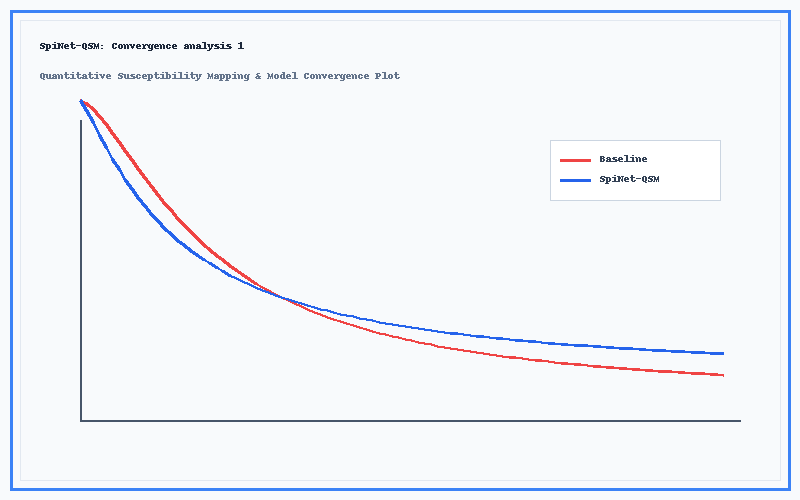
\includegraphics[scale=0.46]{rebuttal_images/Convergence_analysis_1.png}
\caption{\textcolor{black}{Comparison of the convergence for LPCNN and proposed SpiNet-QSM. HFEN, SSIM, and NMSE (computed with respect to COSMOS) for (a)  full training data and (b) limited training data.}}
\label{conv_fig}
\end{figure}


SpiNet-QSM and LPCNN were trained with identical settings to ensure fairness in their comparisons. Both methods used the same CNN architecture (3D-WideResNet-18). \textcolor{black}{To assess convergence, evaluation metrics such as SSIM, HFEN, and NMSE were computed and plotted for each epoch of the test dataset for LPCNN and the proposed SpiNet-QSM.}  \textcolor{black}{ Both models underwent end-to-end training with the number of unrollings, $K=1$, and $K=3$.} 



%-----------------------
\begin{figure*}[htbp]
    \centering
    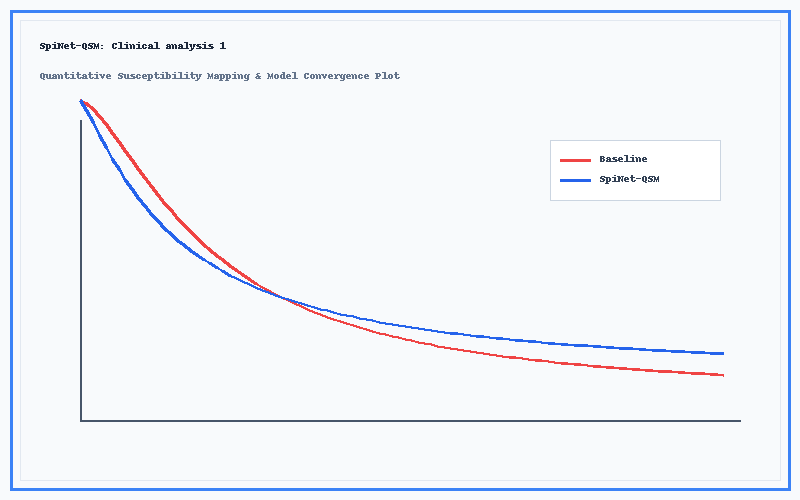
\includegraphics[scale=0.34]{rebuttal_images/Clinical_analysis_1.png}
    \caption{\textcolor{black}{Clinical analysis on hemorrhage and multiple sclerosis (MS) for example cases. The normalized model loss (L2-norm) is shown as insets at the bottom of each image. However, NDI reconstructions for the clinical data were not performed due to the unavailability of magnitude volumes. }}
    \label{fig:galaxy}
\end{figure*}
\section{Results}\label{sec4}


\subsection{Effect of Dataset Size }

\subsubsection{Training on Complete Data}
\textcolor{black}{The quantitative performance metrics such as structural similarity index (SSIM), peak signal to noise ratio (pSNR), normalized mean square error (NMSE), and high-frequency error norm (HFEN) \cite{milovic20202016} with respect to COSMOS of the different QSM reconstruction methods considered in this study are summarized in Table.\ref{tab:results_of_full_data_trained_models}}. One example reconstruction was shown in Fig. \ref{fig:qsm_maps_on_complete_vs_limited}(a). A t-test was performed for statistical analysis, and a statistically significant difference was determined for HFEN, based on a threshold of 0.05. The P-values of SpiNet-QSM matched the results of the deep learning approaches QSMnet (P=0.939), DeepQSM (P=0.372), and xQSM (P=0.505). However, the proposed SpiNet-QSM showed an improvement over the LPCNN approach (P=0.004).
% Figure 6
\begin{figure}[htbp]
    \centering
    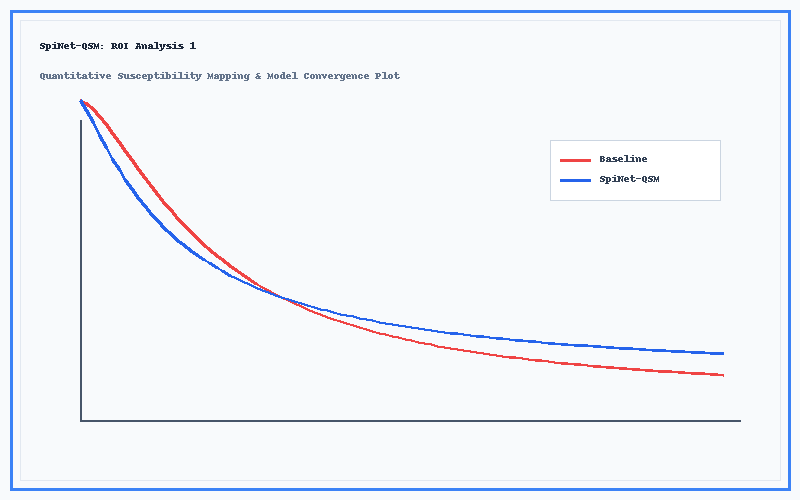
\includegraphics[scale=0.48]{rebuttal_images/ROI_Analysis_1.png}
    \caption{\textcolor{black}{ROI analysis (Caudate, Putamen, and globus pallidus) for an example case. The first row shows the reconstructed susceptibility maps obtained using COSMOS, SpiNet-QSM, LP-CNN, QSMnet, DeepQSM, Star-QSM, and NDI. The second row shows a magnified view of the QSM in the ROI using the above methods. The susceptibility values of Caudate, Putamen, and globus pallidus corresponding to each ROI are shown as insets in the top, middle, and bottom rows, respectively.}}
    \label{fig:ROI_analysis}
\end{figure}

\subsubsection{Training on Limited Data}

\textcolor{black}{The quantitative performance metrics of the different QSM reconstruction methods considered in this study are summarized in Table.\ref{tab:results_of_full_data_trained_models}}. The quality of the reconstructed susceptibility maps was reduced with a reduction in the training data compared with that of the full training data. One example reconstruction was shown in Fig. \ref{fig:qsm_maps_on_complete_vs_limited}(b).  The scatter plots showing the quantitative performance of the proposed as well as other methods were shown in Fig. \ref{fig:scatterplots} both for the complete training data as well as limited training data. From these results, it can be observed that the proposed SpiNet-QSM map matches closely with the gold-standard COSMOS map.
 
 The proposed SpiNet-QSM showed a statistically significant improvement over the existing deep learning approaches, QSMnet ($P=1.16e^{-21}$), DeepQSM ($P=6.23e^{-25}$), and xQSM ($P=7.30e^{-25}$). Even LPCNN performed better than the deep learning methods QSMnet($P=2.42e^{-09}$), DeepQSM ($P=1.4e^{-11}$), and xQSM ($P=4.9e^{-12}$). The performance of NDI also matched that of the deep learning methods QSMnet($P=0.915$), DeepQSM ($P=0.453$), and xQSM ($P=0.202$). For a fair comparison, the proposed SpiNet-QSM and LPCNN approaches were compared with similar training conditions. The proposed SpiNet-QSM showed better reconstruction than the LPCNN ($P=1.27e^{-07}$). 
 

\subsection{Performance on Other Datasets}
\textcolor{black}{
The quantitative metrics obtained from the LPCNN data, RC-1 data, and RC-2 data are summarized in Table. \ref{tab:other_data}. On the LPCNN data, it's evident that the proposed SpiNet-QSM outperforms other approaches. The model-based deep learning method LPCNN and the pure deep learning methods QSMNet, DeepQSM, and xQSM also showed effective QSM reconstruction. Pure deep learning methods achieve comparable performance to LPCNN. Similarly, on the RC-1 data, SpiNet-QSM exhibits superior performance compared to other methods. However, QSMNet, DeepQSM, and xQSM also achieved effective QSM reconstructions. Deep learning methods on RC-1 data match the performance of LPCNN. Both model-based and pure deep learning approaches outperform NDI, an iterative method. On RC-2 data, the iterative method NDI showed better performance than other methods. The Model-based deep learning methods performed closer to that of NDI and, the SpiNet-QSM exhibited slight superiority over the LPCNN. The performance of pure deep learning methods was inferior when compared to the NDI, SpiNet-QSM, and LPCNN. 
Across all three datasets, The model-based deep learning techniques  SpiNet-QSM and LPCNN exhibited consistent performance compared to other deep learning methods. However, SpiNet-QSM showed even better performance than LPCNN.}


\subsection{Convergence Comparison}

\textcolor{black}{Figure \ref{conv_fig} depicts the evaluation metrics versus epochs for both the models. Notably, the plots illustrating the metric improvement show steeper trends in the case of $K=1$. For $K=3$, the weights were initialized to those of $K=1$ for SpiNet-QSM. The saturation observed in SpiNet-QSM metrics with $K=3$ can be attributed to two factors. First, because the weights are initialized with $K=1$, the model is already near the solution space. Second, each epoch of the proposed SpiNet-QSM involves inner iterations, facilitating a faster convergence to the solution. For the LPCNN with $K=3$, the weights initialization from LPCNN with $K=1$ doesn't add any improvement in terms of convergence and performance. SpiNet-QSM consistently outperformed LPCNN in terms of convergence speed, demonstrating its superiority in both full and limited data training scenarios.} \textcolor{black}{The training was stopped for all the methods by considering the model performance on the validation set. SpiNet-QSM with the $K=3$ model converged in the early epochs. However, a minimum of $45$ epochs were considered in the training process.
}\\

\noindent \textcolor{black} {Training one epoch of SpiNet-QSM and LPCNN took $90$ and $120$ minutes, respectively. SpiNet-QSM training was performed for $45$ epochs, which required approximately $68$ hours, and LPCNN training was performed for approximately 80 epochs, required approximately $160$ hours. However, SpiNet-QSM training with $K=3$ was performed by initializing the weights of SpiNet-QSM with $K=1$ (single unrolling). For training one epoch, SpiNet-QSM with $K=1$ took $20$ minutes. The SpiNet-QSM with $K=1$ training was also performed for 50 epochs, which took approximately $17$ hours. By including this training time, the overall training time of SpiNet-QSM with $K=3$ was approximately $85$ hours. Although the LPCNN $K=3$ experiment was attempted by initializing the weights with LPCNN with $K=1$, it did not show any improvement in terms of time and quantitative metrics over the LPCNN with $K=3$ with random default initialization. It should be noted that the model weights were chosen for that epoch when the validation error was the minimum. Remarkably, SpiNet-QSM consistently showed faster convergence than LPCNN.}  



\subsection{Clinical Analysis}



\subsubsection{Testing on Patient Data}
The proposed SpiNet-QSM was tested on clinical data, including hemorrhage and multiple sclerosis (MS), which were not present in the training data. The model loss was utilized to evaluate the performance of the models. One example result from each hemorrhage as well as the MS case was shown in Fig. \ref{fig:galaxy}. 




\subsubsection{ROI Analysis}

The local region susceptibility values (mean and standard deviation) of the three ROIs considered for the six different subjects are summarized in Table \ref{tab:roi_table}. One example set of images were shown in Fig. \ref{fig:ROI_analysis}. The respective COSMOS values are shown for reference. It can be observed that the local measurements of the proposed SpiNet-QSM consistently match with the COSMOS susceptibility measurements.



\section{Discussion }

This study introduces SpiNet-QSM, a model-based deep learning approach for QSM reconstruction. SpiNet-QSM utilizes an unrolling iterative structure with a p-norm-enforced CNN-denoiser-based trainable regularizer, where the regularizer weights are shared across the iterations. However, the inclusion of the regularization term \( \|x - z\|^p_p \) in the SpiNet-QSM objective function makes it non-convex. \textcolor{black}{For the SpiNet-QSM objective function, the majorization-minimization approach was employed, approximating an upper-bound function under conditions where $0 < p \leq 2$. The preference for majorization-minimization \cite{lange2013optimization} over alternatives, such as Gauss-Newton\cite{lange2013optimization,nocedal1999numerical}, is grounded in the challenges posed by non-convex and non-smooth optimization problems. Specifically, the objective function of SpiNet-QSM is nonlinear and can be nonconvex in nature owing to the $p$-norm in the regularization term. For $0 < p < 1$, the regularization term $\|x - z\|^p_p$ is nonconvex. It is also a nonsmooth function at $0 < p < 2$. The Gauss-Newton approach may encounter difficulties in such scenarios, often being prone to convergence issues and becoming trapped in local minima. Majorization-minimization, on the other hand, emerges as a robust choice for handling non-convex and non-smooth functions within the context of the minimization problem. Its iterative nature involves majorizing the objective function using a simpler upper-bound function, thereby making it more suitable for optimization. In contrast to the Gauss-Newton method, majorization-minimization excels in navigating non-convex landscapes, providing effective and consistent performance throughout the optimization process. Each iteration involved refining this upper-bound function to iteratively address the challenges associated with the optimization function. This robustness makes majorization-minimization a practical and reliable approach to this problem.}\\


\noindent \textcolor{black}{Due to the physics-driven nature of SpiNet-QSM and LPCNN, both of them outperformed the existing deep learning methods.} Further, the proposed SpiNet-QSM outperformed LPCNN for both complete and limited data training, despite being trained under similar conditions. \textcolor{black}{Although both the methods use an unrolling iterative structure and a trainable regularizer with weight-sharing, the regularizer term is a direct CNN in the LPCNN approach, whereas it consists of a CNN-based denoiser in SpiNet-QSM. Moreover, SpiNet-QSM enforces the $p$-norm rather than the $2$-norm in LPCNN for the regularizer term, where $ p $ is trainable ($0 < p \le 2$). It was observed from experiments that the converged $p$-value is between 1.5 and 1.8. Thus, in the case of limited data training, the $p$-norm enforced regularizer constrained the proposed SpiNet-QSM to choose a better susceptibility space, enabling the proposed SpiNet-QSM to reconstruct better susceptibility maps. The second distinction lies in the methodology utilized to solve the data consistency part. The proposed SpiNet-QSM solves the data consistency block with the help of the conjugate gradient descent method (as an iterative solver); however, LPCNN uses the proximal gradient method, and in each unrolling, only one proximal gradient step is used. These two factors also helped SpiNet-QSM in achieving faster convergence compared to LPCNN.} However, the end-to-end training of the proposed SpiNet-QSM is computationally more expensive than direct deep learning methods due to the model-based unrolling network architecture. For future improvement, the development of more trainer-friendly networks for model-based deep learning frameworks will be explored.


\section{Conclusion}


In this work, a model-based deep learning framework for single-orientation QSM reconstruction was developed with a Schatten p-norm driven regularizer, where the norm parameter $p$ is trainable.  The proposed SpiNet-QSM is a supervised method for QSM reconstruction with a COSMOS map as the ground truth that uses an unrolled network architecture with shared weights for end-to-end training. The proposed SpiNet-QSM outperformed other state-of-the-art deep learning methods in terms of reconstruction performance with limited training data.  Furthermore, it showed good generalization by yielding robust reconstructions when tested on data collected under different acquisition parameters from those of the training data. The proposed SpiNet-QSM also performed consistently well on clinical data from patients with hemorrhage, multiple sclerosis, and ROI analysis.

\section*{Acknowledgements}

The authors are thankful to Dr. Jongho Lee, Laboratory for Imaging Science and Technology, Department of Electrical and Computer Engineering, Seoul National University, Seoul, South Korea, for providing the data. The authors are also thankful to Dr. Jeremias Sulam, Biomedical Engineering Department, Johns Hopkins University for making their data \cite{lai2020learned} publicly available. The authors are also thankful to Naveen Paluru and Aditya Rastogi, Indian Institute of Science, Bangalore for their input on this work. 

\section*{Data/Code Availability}
 SNU dataset was made available to the authors by Prof. Lee (e-mail:  jonghoyi@snu.ac.kr) of Seoul National University. LPCNN dataset is publicly available at \href{https://github.com/Sulam-Group/LPCNN}{https://github.com/Sulam-Group}\cite{lai2020learned}. 
QSM 2016 reconstruction challenge (RC-1) dataset is publicly available at \href{http://www.neuroimaging.at/pages/qsm.php}{http://www.neuroimaging.at/pages/qsm.php}\cite{langkammer2018quantitative}. QSM reconstruction challenge 2.0 (RC-2) dataset is publicly available at \href{https://doi.org/10.5281/zenodo.4559541}{https://doi.org/10.5281/zenodo.4559541}\cite{marques2021qsm}. The developed codes of this manuscript are publicly shared at \href{https://github.com/venkateshvaddadi/SpiNet-QSM}{https://github.com/venkateshvaddadi/SpiNet-QSM}.



\bibliography{sn-bibliography}
%\bibliographystyle{unsrt}
\end{document}
